\section{The {\em paṇḍaka}}

After having looked at the references and descriptions of the word {\em paṇḍaka} in Vedic text, Jain discussions and Buddhist scriptures of both Pāli and Chinese origin, a clearer picture emerges of what the {\em paṇḍaka} really is and what the reasons are behind the Buddhist rules against ordination.

As we have seen, the oldest emergence of the {\em paṇḍaka} and the {\em klība} as sub-categories of the {\em napuṃsaka} ('neither male nor female') happened in Vedic times. They are the 'un-males', the 'impotent', destined from birth to play a role in the larger fabric of Indian religion, society and culture. They are the embodiment of the feminine in the masculine, a living myth. They are categorised by their feminine behavior and dress, their impotence, their occupation as religious dancers and singers and their emasculation. They are there to remind us of the deeply ambivalent attitude of men towards women and women's sexuality, their desire for, and at the same time their fear of the feminine.

With the emergence of the Jain ascetics a debate started with regards to the position of women in the order, and as a consequence the position of the {\em napuṃsaka}. This discussion necessitated the identification of the characteristics that make up a male, a female and by consequence a {\em napuṃsaka}. We see that a similar discussion was held among the Buddhists\footnote{\cite{sujato2009}}, especially after the Buddha himself passed away and the order found itself without a leader. This discussion was also fuelled by the public opinion of the celibate monastics. We know from both the Buddhist Suttas as the Jain scriptures that debates were also held between the Jains and Buddhists about a variety of subjects and no doubt there was an influence between these orders.

As a result the Buddhist Vinaya was redacted during the Second Council. It is not so far-fetched to infer that if the Vinaya was redacted with regards to women's ordination, the position of the {\em paṇḍaka} was also laid down at this time\footnote{Before this time we have no reference of the {\em paṇḍaka} in the Early Buddhist Suttas as shown in \ref{pali1}; the term is only used in the Vinaya and later commentarial texts}. This is when we see the emergence of the {\em paṇḍaka} as the hyperlibidous effeminate male who seduces monks and lay men alike, who is unable to maintain his precepts and who can, by his very nature, not be a monk. This idea of the hyperlibidousness of the {\em paṇḍaka} because he possesses both male and female {\em veda} we have also seen in the Jain scriptures. But there is no further explanation of what the {\em paṇḍaka} really is and what his characteristics are until later, when the five types of {\em paṇḍaka} are defined. 

At this point in time the Jain and Buddhist scriptures and their development begin to diverge as schools begin to emerge after King Ahsoka has sent his missionaries to different parts of his empire. The Jain also begin to create subdivisions of the {\em napuṃsaka}, but the {\em paṇḍaka} is not further divided and remains as a person who cannot ordain. 

The Buddhist scriptures are dispersed and eventually translated into Chinese in the various schools. There the word {\em paṇḍaka} was first translated as 'impotent' (種不能男) and later as 'eunuch' (黃門). The translation 'eunuch' however was taken from the word 'yellow gate', denoting the Han Dynasty imperial palace eunuchs. This was possibly the only way that the Chinese could relate to a {\em paṇḍaka}, being unfamiliar with the rich religious concept that they embody. It is clear that the Chinese palace eunuchs cannot be compared to the hijra from India.

\begin{figure}[!tbp]
  \centering
  \subfloat[Palace eunuchs in ancient China]{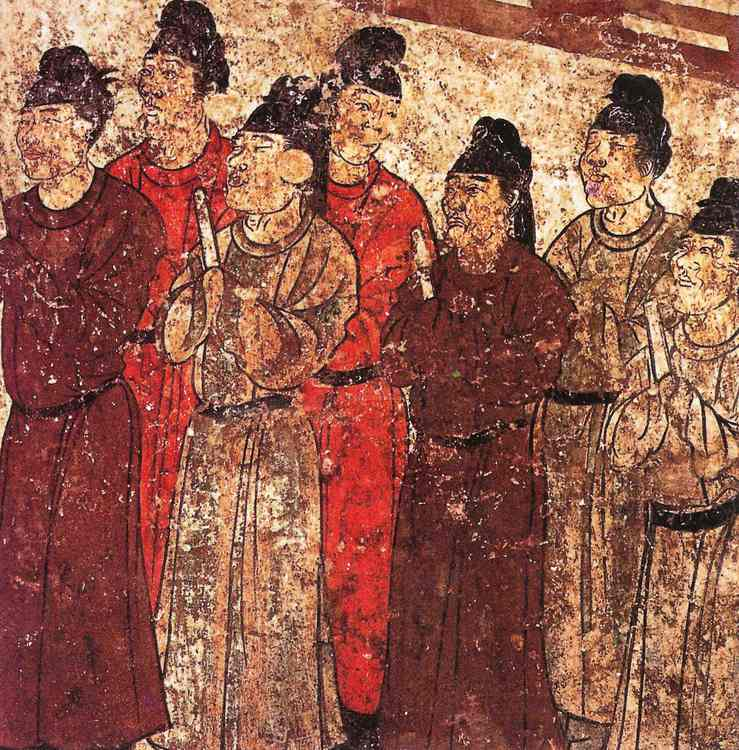
\includegraphics[width=0.4\textwidth]{Eunuchs-in-ancient-China.jpg}}
  \hfill
  \subfloat[Hijra in India]{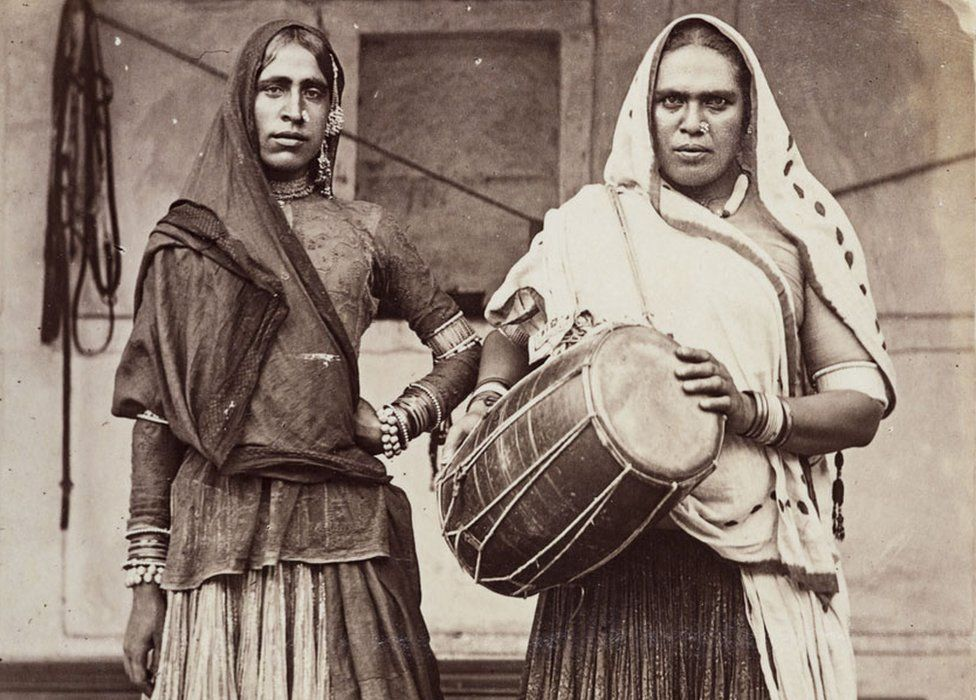
\includegraphics[width=0.4\textwidth]{hijra.jpg}}
\end{figure}

Moreover, the castrated {\em paṇḍaka} i.e. a eunuch, is only one type of the five types that cannot ordain, which makes it highly unlikely that the word {\em paṇḍaka} means 'eunuch'. We would also not expect a eunuch to have hyperlibidousness. After all, castrated men were often employed as harem guards just for the reason that they are no longer interested in sexual activity and therefore considered safe. Moreover, the Dharmaguptaka Vinaya treats the castrated man as something other than a {\em paṇḍaka}.

To fully understand the types of {\em paṇḍaka} in the scriptures, we have to look again at the understanding of the gender roles at that time. Whether or not the {\em paṇḍaka} in form of the religious embodiment of the feminine in the masculine was already engaged in prostitution at the time of the Buddha or not, in any case he was seen to have the female {\em veda} simply because he was "not a male". He dressed and behaved like a woman, a temptress that could arouse desire in the celebate monk. 

As we have seen in the Jain scriptures, the discussion to overcome the ambiguities in the understanding of the word {\em paṇḍaka} resulted over time in changes in meaning and use and the definition of sub-categories. I believe that it is likely that the term {\em opakkamikapaṇḍaka} represented castrated man, the {\em klība}, or the initiated hijra, while the {\em napuṁsakapaṇḍaka} was the re-definition of the original {\em paṇḍaka}, the still uninitiated hijra, or the 'female {\em napuṃsaka}' that we saw emerging in the Jain commentarial texts.

The {\em pakkhapaṇḍaka} is interesting and several explations have been given by authors over time, none of which I find convincing. As we can still understand the meaning of the other four categories and understand their meaning in light of people's physiology or sexual fetishes, the "half-moon" {\em paṇḍaka} is an enigma. Turning back to the Vedic texts however, we find in the {\em Uttarakanda} of the {\em Rāmāyaṇam}\footnote{Rām 7.78-79. See also \cite{goldman}} the story of King Ila. In this epic tale the king accidentally stumbles upon the Mother Goddess in intimate embrace with Śiva, who turn him into a woman. Now Ilā, she turns to the Goddess for mercy to restore her manhood but is only granted half her wish; namely that she has to change sex each month. With the change of sex also comes a change in sexual desire. As a woman she falls in love, becomes pregnant and gives birth, reverting back and forth between male and female. The theme of changing genders based on the phases of the moon is a recurrent theme in the Vedic myths and it is not unlikely that this mythical theme has found it's way into the Vinaya in the form of the {\em pakkhapaṇḍaka}. After all, another rule in the Vinayas of all the schools tells the tale of a shape-shifting serpent, a mythological beast, a {\em Nāga}, who ordains as a monk, is later discovered and a new rule is laid down in much the same manner as for the {\em paṇḍaka}, barring him and all his kind from ordination. The fabric of myth and reality can easily overlap in Indian culture.

As for the other two, the {\em āsittapaṇḍaka} and the {\em usūyapaṇḍaka}, who at least in the {\em Theravāda} tradition are allowed to ordain, I believe they embody another of the Jain categories, namely the category of the {\em puruṣanapuṃsaka} (male {\em napuṃsaka}). Although they might be impotent and are therefore also in possession of the female {\em veda}, they can "pass" as a man an therefore not only appear as men to the lay supporters but also to the celibate monks they live with who are not arroused by their presence. The relaxation of the rules for these two types also runs parallel with the development in the Jain scriptures. But unlike the Jain, no further abolishment of this entire rule against the ordination of {\em paṇḍaka} was reached simply because the Buddhist scriptures were closed while the Jain scriptures continued to evolve for many centuries thereafter.







For ubhatojanaka:

\cite{goldman} In the story of King Ila as told in the {\em Uttarakanda} of the {\em Rāmāyaṇam}\footnote{Rām 7.78-79}, the king accidentally stumbles upon the Mother Goddess in intimate embrace with Śiva, who turn him into a woman. Now Ilā, she turns to the Goddess for mercy to restore her manhood but is only granted half her wish; namely that she has to change sex each month. With the change of sex also comes a change in sexual desire. As a woman she falls in love, becomes pregnant and gives birth, reverting back and forth between male and female. 

From the statistical analysis in \ref{appendix2} we can see that the sanskrit texts follow the Pali in that no mention is made of {\em ubhayavyañjana} in the sutras. Just like in the pali, we only find the word in the later texts and Vinaya. What is more interesting is that the word is not found in the pre-Buddhist texts or later Brahmanical texts. This raises questions as to the origin of the word, of which not much seems to be known.

Considering that the literal meaning of the word {\em ubhayavyañjana} is "having the characteristics of both sexes"\footnote{\href{https://suttacentral.net/define/ubhatovya%C3%B1janaka}{The definition in the New Concise Pali English Dictionary} defines the term as "having the sexual characteristics of both sexes; hermaphrodite". But the literal meaning of the term says nothing about the characteristics needing to be sexual in origin; {\em ubhato} meaning "in both ways, on both sides" and {\em byañjana} or {\em vyañjana} means "sign or mark". As the term "hermaphrodite" is nowadays only used for species that can reproduce both as male and female, I discard this translation.}, we could postulate that the word is a synomym of {\em napuṃsaka} or at least a class of {\em napuṃsaka}. As we have also seen that the Buddhist texts seem to follow the Brahmanical idea of gender-characteristics or {\em liṅga}, this seems to underline this postulation.


----------------------------------------


\section{Buddhist views on the third sex}
The Buddhist view as mentioned in the Abhidharma Kośa (IV.14c) (4–5th century CE) approximates that of the Brahmanical view that sex ({\em vyañjana}) is distinguised on the basis of primary and secondary sexual characteristics.

In the early Buddhist Pāli texts, we find remarkably little on the subject, but in later commentaries and Mahāyāna texts we find a number of recognized third sex types that are discussed in more detail, defined also based on their sexual behavior and not only on their external characteristics. As Buddhist monks did not go naked, and in fact identified themselves as different from Jains by the fact that they had a bowl and robe, this issue might have been less important than for the Jain.


(CLAIRE's ESSAY ON THIS)
(THE DISCUSSION BIT IN HERE)




Religious groups also formed their own vocabulary like for instance the the Jain did not use the Brahmanical standard term {\em liṅga} for gender-characteristics but introduced their own term {\em veda}. It is not unlikely that the Buddhists also formed their own vocabulary\footnote{In the suttas also we find instances where the Buddhists use different terms for the same things as the Jains. Majjhima Nikāya 56 recounts a discussion between the Buddha and the Jain ascetic Tapassī in which the ascetic says: {\em “Na kho, āvuso gotama, āciṇṇaṃ nigaṇṭhassa nāṭaputtassa ‘kammaṃ, kamman’ti paññapetuṃ; ‘daṇḍaṃ, daṇḍan’ti kho, āvuso gotama, āciṇṇaṃ nigaṇṭhassa nāṭaputtassa paññapetun”ti.} “Reverend Gotama, Nigaṇṭha Nātaputta {\em (i.e. Mahāvīra)} doesn’t usually speak in terms of ‘deeds’ He usually speaks in terms of ‘rods’.” }. and used the term {\em ubhayavyañjana} instead of {\em napuṃsaka}. In Buddhism we also find the term {\em napuṃsaka} in the commentarial and later texts only.


The {\em klība} is notable for it's absense in the Buddhist canon. Considering that this is defined as a man whose penis is destroyed, it could also have been taken as synomym of {\em paṇḍaka}, even though it is treated as different in the Sanskrit Vedas and Brahmanical texts.

linga also mainly appear in the commentarial texts in the pali.